\documentclass[border=8pt, multi, tikz]{standalone}
\usetikzlibrary{positioning,fit,arrows.meta}
\usepackage{amsmath,amssymb}

\definecolor{datacol}{RGB}{214,239,216}
\definecolor{netcol}{RGB}{222,226,255}
\definecolor{stdcol}{RGB}{255,243,205}
\definecolor{priorcol}{RGB}{255,224,230}
\definecolor{mcmccol}{RGB}{224,247,250}
\definecolor{postcol}{RGB}{240,224,255}

\begin{document}
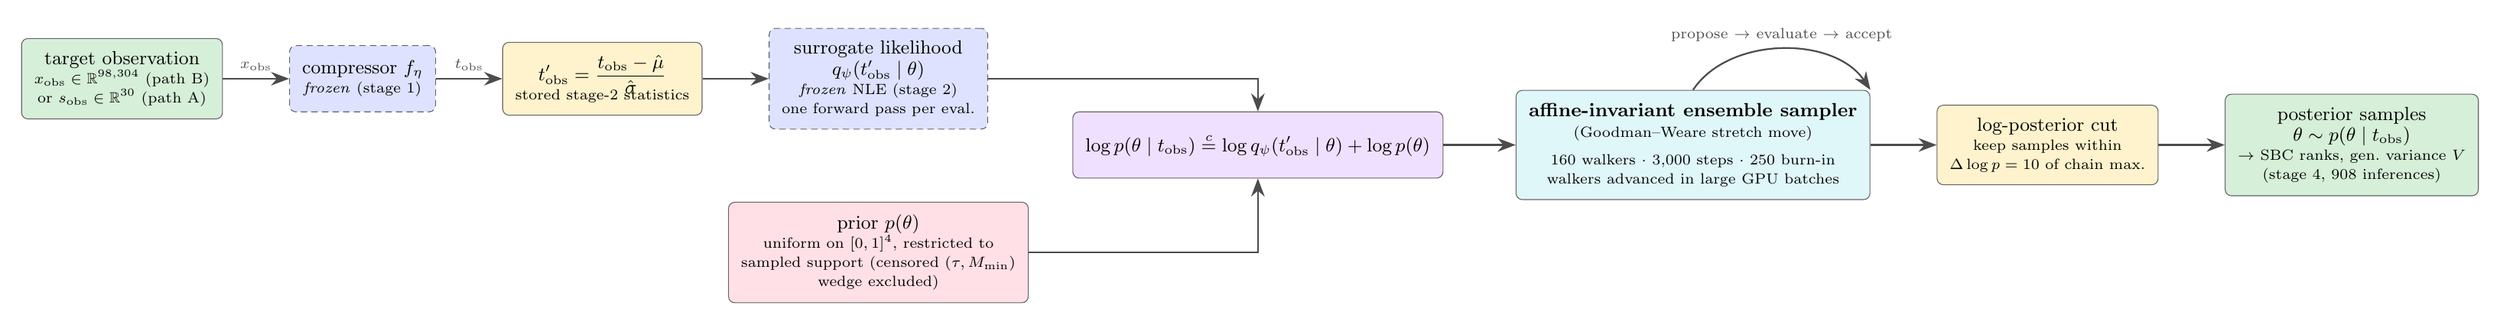
\begin{tikzpicture}[
  node distance=8mm and 11mm,
  every node/.style={font=\small},
  box/.style={draw=black!60, rounded corners=3pt, align=center, inner sep=6pt, minimum height=11mm},
  frozen/.style={box, fill=netcol, densely dashed},
  arr/.style={-{Stealth[length=3mm]}, thick, black!70}
]

% ---------------- top row: observation -> summary -> likelihood ----------------
\node[box, fill=datacol] (obs) {target observation\\[-2pt]\scriptsize $x_{\mathrm{obs}}\in\mathbb{R}^{98{,}304}$ (path B)\\[-2pt]\scriptsize or $s_{\mathrm{obs}}\in\mathbb{R}^{30}$ (path A)};

\node[frozen, right=of obs] (comp) {compressor $f_\eta$\\[-2pt]\scriptsize \emph{frozen} (stage 1)};

\node[box, fill=stdcol, right=of comp] (std) {$t'_{\mathrm{obs}} = \dfrac{t_{\mathrm{obs}}-\hat\mu}{\hat\sigma}$\\[-2pt]\scriptsize stored stage-2 statistics};

\node[frozen, right=of std] (nle) {surrogate likelihood\\[-1pt]$q_\psi(t'_{\mathrm{obs}}\mid\theta)$\\[-2pt]\scriptsize \emph{frozen} NLE (stage 2)\\[-2pt]\scriptsize one forward pass per eval.};

% ---------------- prior ----------------
\node[box, fill=priorcol, below=12mm of nle] (prior) {prior $p(\theta)$\\[-2pt]\scriptsize uniform on $[0,1]^4$, restricted to\\[-2pt]\scriptsize sampled support (censored $(\tau, M_{\min})$\\[-2pt]\scriptsize wedge excluded)};

% ---------------- posterior kernel ----------------
\node[box, fill=postcol, right=14mm of nle, yshift=-11mm] (logp)
  {$\log p(\theta\mid t_{\mathrm{obs}}) \overset{c}{=} \log q_\psi(t'_{\mathrm{obs}}\mid\theta) + \log p(\theta)$};

% ---------------- sampler ----------------
\node[box, fill=mcmccol, right=12mm of logp, minimum width=52mm] (mcmc)
  {\textbf{affine-invariant ensemble sampler}\\[-1pt]
   \scriptsize (Goodman--Weare stretch move)\\[2pt]
   \scriptsize 160 walkers $\cdot$ 3{,}000 steps $\cdot$ 250 burn-in\\[-2pt]
   \scriptsize walkers advanced in large GPU batches};

% self-loop: propose / evaluate / accept
\draw[arr] (mcmc.north) .. controls +(0.6,0.9) and +(-0.6,0.9) .. node[above, font=\scriptsize]{propose $\to$ evaluate $\to$ accept} (mcmc.north east);

% ---------------- post-processing ----------------
\node[box, fill=stdcol, right=of mcmc] (filt) {log-posterior cut\\[-2pt]\scriptsize keep samples within\\[-2pt]\scriptsize $\Delta\log p = 10$ of chain max.};

\node[box, fill=datacol, right=of filt] (post) {posterior samples\\[-1pt]$\theta \sim p(\theta\mid t_{\mathrm{obs}})$\\[-2pt]\scriptsize $\to$ SBC ranks, gen.\ variance $V$\\[-2pt]\scriptsize (stage 4, 908 inferences)};

% ---------------- arrows ----------------
\draw[arr] (obs) -- node[above, font=\scriptsize]{$x_{\mathrm{obs}}$} (comp);
\draw[arr] (comp) -- node[above, font=\scriptsize]{$t_{\mathrm{obs}}$} (std);
\draw[arr] (std) -- (nle);
\draw[arr] (nle.east) -| (logp.north);
\draw[arr] (prior.east) -| (logp.south);
\draw[arr] (logp) -- (mcmc);
\draw[arr] (mcmc) -- (filt);
\draw[arr] (filt) -- (post);

\end{tikzpicture}
\end{document}
